\documentclass{beamer}
\usepackage[utf8]{inputenc}

\usetheme{Madrid}
\usecolortheme{default}
\usepackage{amsmath,amssymb,amsfonts,amsthm}
\usepackage{txfonts}
\usepackage{tkz-euclide}
\usepackage{listings}
\usepackage{adjustbox}
\usepackage{array}
\usepackage{tabularx}
\usepackage{gvv}
\usepackage{lmodern}
\usepackage{circuitikz}
\usepackage{tikz}
\usepackage{graphicx}

\setbeamertemplate{page number in head/foot}[totalframenumber]

\usepackage{tcolorbox}
\tcbuselibrary{minted,breakable,xparse,skins}



\definecolor{bg}{gray}{0.95}
\DeclareTCBListing{mintedbox}{O{}m!O{}}{%
	breakable=true,
	listing engine=minted,
	listing only,
	minted language=#2,
	minted style=default,
	minted options={%
		linenos,
		gobble=0,
		breaklines=true,
		breakafter=,,
		fontsize=\small,
		numbersep=8pt,
		#1},
	boxsep=0pt,
	left skip=0pt,
	right skip=0pt,
	left=25pt,
	right=0pt,
	top=3pt,
	bottom=3pt,
	arc=5pt,
	leftrule=0pt,
	rightrule=0pt,
	bottomrule=2pt,
	toprule=2pt,
	colback=bg,
	colframe=orange!70,
	enhanced,
	overlay={%
		\begin{tcbclipinterior}
			\fill[orange!20!white] (frame.south west) rectangle ([xshift=20pt]frame.north west);
	\end{tcbclipinterior}},
	#3,
}
\lstset{
	language=C,
	basicstyle=\ttfamily\small,
	keywordstyle=\color{blue},
	stringstyle=\color{orange},
	commentstyle=\color{green!60!black},
	numbers=left,
	numberstyle=\tiny\color{gray},
	breaklines=true,
	showstringspaces=false,
}
\begin{document}

\title 
{1.5.28}
\date{August 26,2025}

\author 
{Naman kumar-EE25BTECH11041}
\graphicspath{./figs}


\frame{\titlepage}
\begin{frame}{Question}
$\Vec{P} (5, -3)$ and $\Vec{Q}$ (3, y) are the points of trisection of the line segment joining $\Vec{A} (7, -2)$ and $\Vec{B} (1, -5)$. Then y equals.
\end{frame}

\begin{frame}{Equation Used}
\begin{align}
\Vec{Q}=\frac{1}{1+k}\brak{\Vec{A}+k\Vec{B}}
\end{align}
\end{frame}

\begin{frame}{Theoratical Solution}
\begin{align}
\Vec{Q}=\frac{1}{1+2}\brak{\myvec{7\\-2}+2\myvec{1\\-5}}\\
\Vec{Q}=\frac{1}{1+2}\brak{\myvec{9\\-12}}\\
\Vec{Q}=\myvec{3\\-4}\\
\Vec{Q}=\myvec{3\\y}=\myvec{3\\-4}
\end{align}

Therefore, value of y = 4
\end{frame}


\begin{frame}[fragile]
\frametitle{C Code - Section formula function }
\begin{lstlisting}
#include <stdio.h>

void trisec(double k, double x1, double y1, double x2, double y2, double* a, double* b){
    *a= (x1+k*x2)/(1+k);
    *b= (y1+k*y2)/(1+k);
}
\end{lstlisting}
    
\end{frame}

\begin{frame}[fragile]
\frametitle{Python Code through shared output}
\begin{lstlisting}
import ctypes
import numpy as np
import matplotlib.pyplot as plt

# --- Ctypes Setup ---

# Load the shared library. 
# Make sure 'main.so' is in the same directory as this Python script,
# or provide the full path to it.
try:
    c_lib = ctypes.CDLL('./main.so')
except OSError as e:
    print(f"Error loading shared library: {e}")
    print("Please ensure 'main.so' is in the same directory as this script.")
    exit()

# Define the argument types for the C function.
\end{lstlisting}
\end{frame}

\begin{frame}[fragile]
\frametitle{Python Code through shared output}
\begin{lstlisting}
# The C function signature is:
# void trisec(double x1, double y1, double x2, double y2, double* a, double* b, double* c, double* d)
c_lib.trisec.argtypes = [
    ctypes.c_double, 
    ctypes.c_double, 
    ctypes.c_double,
    ctypes.c_double, 
    ctypes.c_double, 
    ctypes.POINTER(ctypes.c_double), 
    ctypes.POINTER(ctypes.c_double)
]

# Define the return type of the function.
c_lib.trisec.restype = None

# --- Calculation ---
\end{lstlisting}
\end{frame}

\begin{frame}[fragile]
\frametitle{Python Code through shared output}
\begin{lstlisting}

# Define the input coordinates for the two endpoints of the line segment

k = 2
x1, y1 = 7.0, -2.0
x2, y2 = 1.0, -5.0

# Prepare ctypes variables to hold the results.
# These will act as the pointers that the C function will write to.
ta = ctypes.c_double()
tb = ctypes.c_double()

# Call the C function from Python to calculate the trisection point
c_lib.trisec(k, x1, y1, x2, y2, ctypes.byref(ta), ctypes.byref(tb))
\end{lstlisting}
\end{frame}

\begin{frame}[fragile]
\frametitle{Python Code through shared output}
\begin{lstlisting}

# Extract the float values from the ctypes variables
ta_val, tb_val = ta.value, tb.value
print(f"Line segment from ({x1}, {y1}) to ({x2}, {y2})")
print(f"Trisection point 1 calculated by C code: ({ta_val:.2f}, {tb_val:.2f})")

# --- Plotting ---

# Create the plot
plt.figure(figsize=(8, 6))

# Plot the full line segment
plt.plot([x1, x2], [y1, y2], 'g--', label="Line Segment")

# Plot the endpoints of the line
plt.scatter([x1, x2], [y1, y2], color="red", s=100, zorder=5, label="Endpoints")
\end{lstlisting}
\end{frame}

\begin{frame}[fragile]
\frametitle{Python Code through shared output}
\begin{lstlisting}
plt.text(x1, y1 - 0.5, f"A ({x1:.1f}, {y1:.1f})", color="red", fontsize=10)
plt.text(x2, y2 - 0.5, f"B ({x2:.1f}, {y2:.1f})", color="red", fontsize=10)

# Plot the calculated trisection point
plt.scatter(ta_val, tb_val, color="blue", marker="X", s=150, zorder=5, label="Trisection Point")
plt.text(ta_val, tb_val + 0.3, f"Trisection Pt 1\n({ta_val:.2f}, {tb_val:.2f})", color="blue", fontsize=10)

# Configure plot appearance
plt.title("Line Segment and its Trisection Point")
plt.xlabel("X-axis")
plt.ylabel("Y-axis")
plt.legend(loc="upper left")
plt.grid(True)
plt.axis("equal") # Ensures the scaling is the same on both axes
plt.show()


\end{lstlisting}
\end{frame}

\begin{frame}[fragile]
\frametitle{Python Code: Direct}
\begin{lstlisting}
import matplotlib.pyplot as plt
import numpy as np

# --- Function Definition (similar to the C code) ---
# This function calculates the coordinates (a, b) of a point that divides
# the line segment from (x1, y1) to (x2, y2) in the ratio k:1.
# This is derived from the section formula: (n*x1 + m*x2)/(m+n)
# by setting the ratio as k = m/n.
def trisec(k, x1, y1, x2, y2):
    """
    Calculates the coordinates of a point dividing a line segment.
    
    Args:
        k (float): The ratio m/n for the section formula.
        x1, y1 (float): Coordinates of the first point (A).
        x2, y2 (float): Coordinates of the second point (B).
\end{lstlisting}
\end{frame}

\begin{frame}[fragile]
\frametitle{Python Code: Direct}
\begin{lstlisting}
    Returns:
        tuple: A tuple containing the (x, y) coordinates of the dividing point.
    """
    a = (x1 + k * x2) / (1 + k)
    b = (y1 + k * y2) / (1 + k)
    return (a, b)

# --- Problem Setup ---
# Given points for the line segment
A = (7, -2)
B = (1, -5)

# --- Calculations ---
# The points of trisection divide the segment in ratios 1:2 and 2:1.

# 1. Calculate Point P (divides AB in ratio 1:2)
\end{lstlisting}
\end{frame}

\begin{frame}[fragile]
\frametitle{Python Code: Direct}
\begin{lstlisting}
# Here, m=1, n=2, so k = m/n = 1/2 = 0.5
k_p = 0.5
P_calculated = trisec(k_p, A[0], A[1], B[0], B[1])

# 2. Calculate Point Q (divides AB in ratio 2:1)
# Here, m=2, n=1, so k = m/n = 2/1 = 2.0
k_q = 2.0
Q_calculated = trisec(k_q, A[0], A[1], B[0], B[1])

y_solution = Q_calculated[1]

# --- Output the Results to Console ---
print("--- Trisection Calculation ---")
print(f"Point A: {A}")
print(f"Point B: {B}\n")

print(f"Calculated coordinates for P (ratio 1:2, k={k_p}): {P_calculated}")
\end{lstlisting}
\end{frame}

\begin{frame}[fragile]
\frametitle{Python Code: Direct}
\begin{lstlisting}
print(f"Calculated coordinates for Q (ratio 2:1, k={k_q}): {Q_calculated}\n")

print("--- Solution ---")
print(f"The problem states Q is (3, y). Our calculation gives Q as {Q_calculated}.")
print(f"Therefore, the value of y is {int(y_solution)}.")
plt.figure(figsize=(10, 8))
ax = plt.gca()

plt.plot([A[0], B[0]], [A[1], B[1]], 'b-', label='Line Segment AB', zorder=1)
points = {'A': A, 'B': B, 'P': P_calculated, 'Q': Q_calculated}
\end{lstlisting}
\end{frame}

\begin{frame}[fragile]
\frametitle{Python Code: Direct}
\begin{lstlisting}
colors = {'A': 'red', 'B': 'red', 'P': 'green', 'Q': 'green'}
for name, (px, py) in points.items():
    plt.scatter(px, py, color=colors[name], s=100, zorder=2)
    plt.text(px + 0.1, py + 0.1, f'{name}({px:.1f}, {py:.1f})', fontsize=12)

plt.xlabel('X-axis', fontsize=12)
plt.ylabel('Y-axis', fontsize=12)
ax.set_aspect('equal', adjustable='box')
plt.grid(True, linestyle='--', alpha=0.6)
plt.legend()
plt.xlim(0, 8)
plt.ylim(-6, 0)

plt.savefig('trisection_diagram.png')
print("\nDiagram saved as 'trisection_diagram.png'")
plt.show()

\end{lstlisting}
\end{frame}

\begin{frame}{Graph}
    \begin{figure}
        \centering
        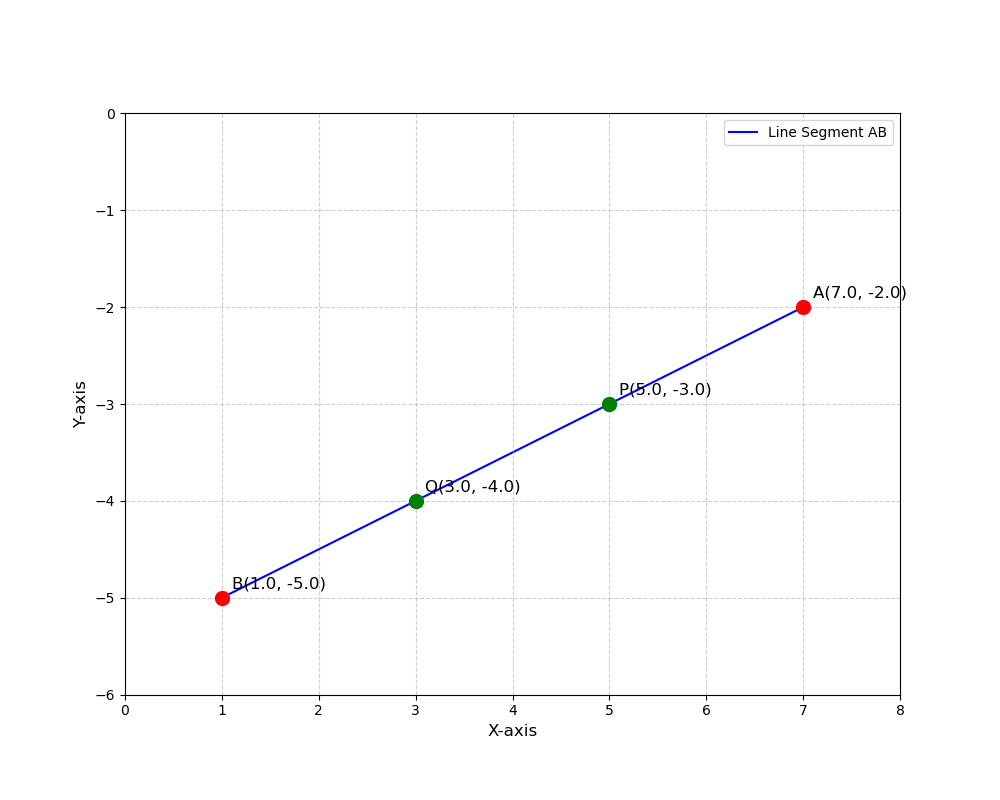
\includegraphics[width=0.9\columnwidth]{figs/trisection_diagram.png}
    \end{figure}
\end{frame}

\end{document}